\section{基本的な計算}
\subsection{起動と使い方}
通常 \verb+>+ が表示されており,入力待ちの状態である.式や関数を入力しEnterを押せば計算結果が表示される.
\begin{breakbox}
\begin{verbatim}
> 1 + 2
[1] 3
> (1 + 2i) * (1 - 2i)
[1] 5+0i
> sum(1:10)
[1] 55
> rep(1, 10)
[1] 1 1 1 1 1 1 1 1 1 1
> seq(1,5, 0.5)
[1] 1.0 1.5 2.0 2.5 3.0 3.5 4.0 4.5 5.0
> ubuntu <- c(1, 2, 3, 4, 5, 6)
> ubuntu
[1] 1 2 3 4 5 6
# コメントアウトは # です.
\end{verbatim}
\end{breakbox}
代入演算子は \verb+<-+,\verb+=+,\verb+->+ が用意されている.推奨は \verb+<-+ である.
\begin{description}
\item[四則演算の演算子]\mbox{}
\begin{table}[H]
\begin{center}
% \caption{表}
\vspace{1zw}
\label{03AB-A2}
\begin{tabular}{c|c}
\noalign{\hrule height 1pt}
演算子&意味\\ \hline
{\tt +}&足し算\\
\verb+^+&累乗\\
\verb+-+&引き算\\
\verb+%/%+&整数商\\
\verb+*+&掛け算\\
\verb+%%+&剰余\\
\verb+/+&割り算\\
\noalign{\hrule height 1pt}
\end{tabular}
\end{center}
\end{table}
\item[特殊な演算子]\mbox{}
\begin{table}[H]
\begin{center}
% \caption{表}
\vspace{1zw}
\label{03AB-A2}
\begin{tabular}{c|c}
\noalign{\hrule height 1pt}
演算子&意味\\ \hline
\verb+:+&公差$\pm$1の数列の作成\\
\verb+%*%+&行列積\\
\verb+%o%+&外積\\
\verb+[ ]+&配列や行列の要素の取出し\\
\verb+[[ ]]+&リスト成分の取出し\\
\verb+$+&データフレーム内の変数の取出し\\
\noalign{\hrule height 1pt}
\end{tabular}
\end{center}
\end{table}
\end{description}

オブジェクトの名前は予約語(すでに基本的な関数で使われている名前)でなければ使用できる.演算子を使うことや名前の最初に数字や\verb+_+(アンダーバー)を使うことはできない.必要であれば \verb+.+(ドット)か \verb+_+(アンダーバー) を使用する.ちなみに日本語も使用可能ではあるが,対応していないライブラリがあるので使用にはあまり適さない.
前に使った命令は入力時にキーボードの「↑」を押すと履歴をさかのぼることができる.
\begin{breakbox}
\begin{verbatim}
> 2 * ubuntu
[1]  2  4  6  8 10 12
> 大学 = "univ"
> 大学
[1] "univ"
> debian = matrix(1:12, 3, 4)
> debian
     [,1] [,2] [,3] [,4]
[1,]    1    4    7   10
[2,]    2    5    8   11
[3,]    3    6    9   12
> matrix(1:12, 3, 4, byrow = T)
     [,1] [,2] [,3] [,4]
[1,]    1    2    3    4
[2,]    5    6    7    8
[3,]    9   10   11   12
> t(debian)
     [,1] [,2] [,3]
[1,]    1    2    3
[2,]    4    5    6
[3,]    7    8    9
[4,]   10   11   12
> debian * debian
     [,1] [,2] [,3] [,4]
[1,]    1   16   49  100
[2,]    4   25   64  121
[3,]    9   36   81  144
> debian %*% t(debian)
     [,1] [,2] [,3]
[1,]  166  188  210
[2,]  188  214  240
[3,]  210  240  270
> ubuntu[3]
[1] 3
> debian[2, ]
[1]  2  5  8 11
> debian[, 3]
[1] 7 8 9
> debian[2, 3]
[1] 8
\end{verbatim}
\end{breakbox}

四則演算の演算子では,要素のそれぞれが計算され,行列の積は計算できない.

この{\tt matrix}関数では\verb+matrix(行列の要素, 行の数, 列の数, …)+というようにオプション引数が存在する.この引数を確認するには\verb+args(matrix)+と入力することで確認できる.
\begin{breakbox}
\begin{verbatim}
> args(matrix)
function (data = NA, nrow = 1, ncol = 1, byrow = FALSE, dimnames = NULL) 
NULL
\end{verbatim}
\end{breakbox}

{\tt args}関数を使用することで引数の名前がわかるが,引数の名前だけでは,必要な情報がそろわない場合がある.そのような場合は,ヘルプページを表示すればよい.
\begin{breakbox}
\begin{verbatim}
> ?matrix
starting httpd help server ... done
> help(matrix)
\end{verbatim}
\end{breakbox}

以下の,マニュアルが表示される.関数の説明や使い方,引数,例などが英語で記されている.
\begin{center}
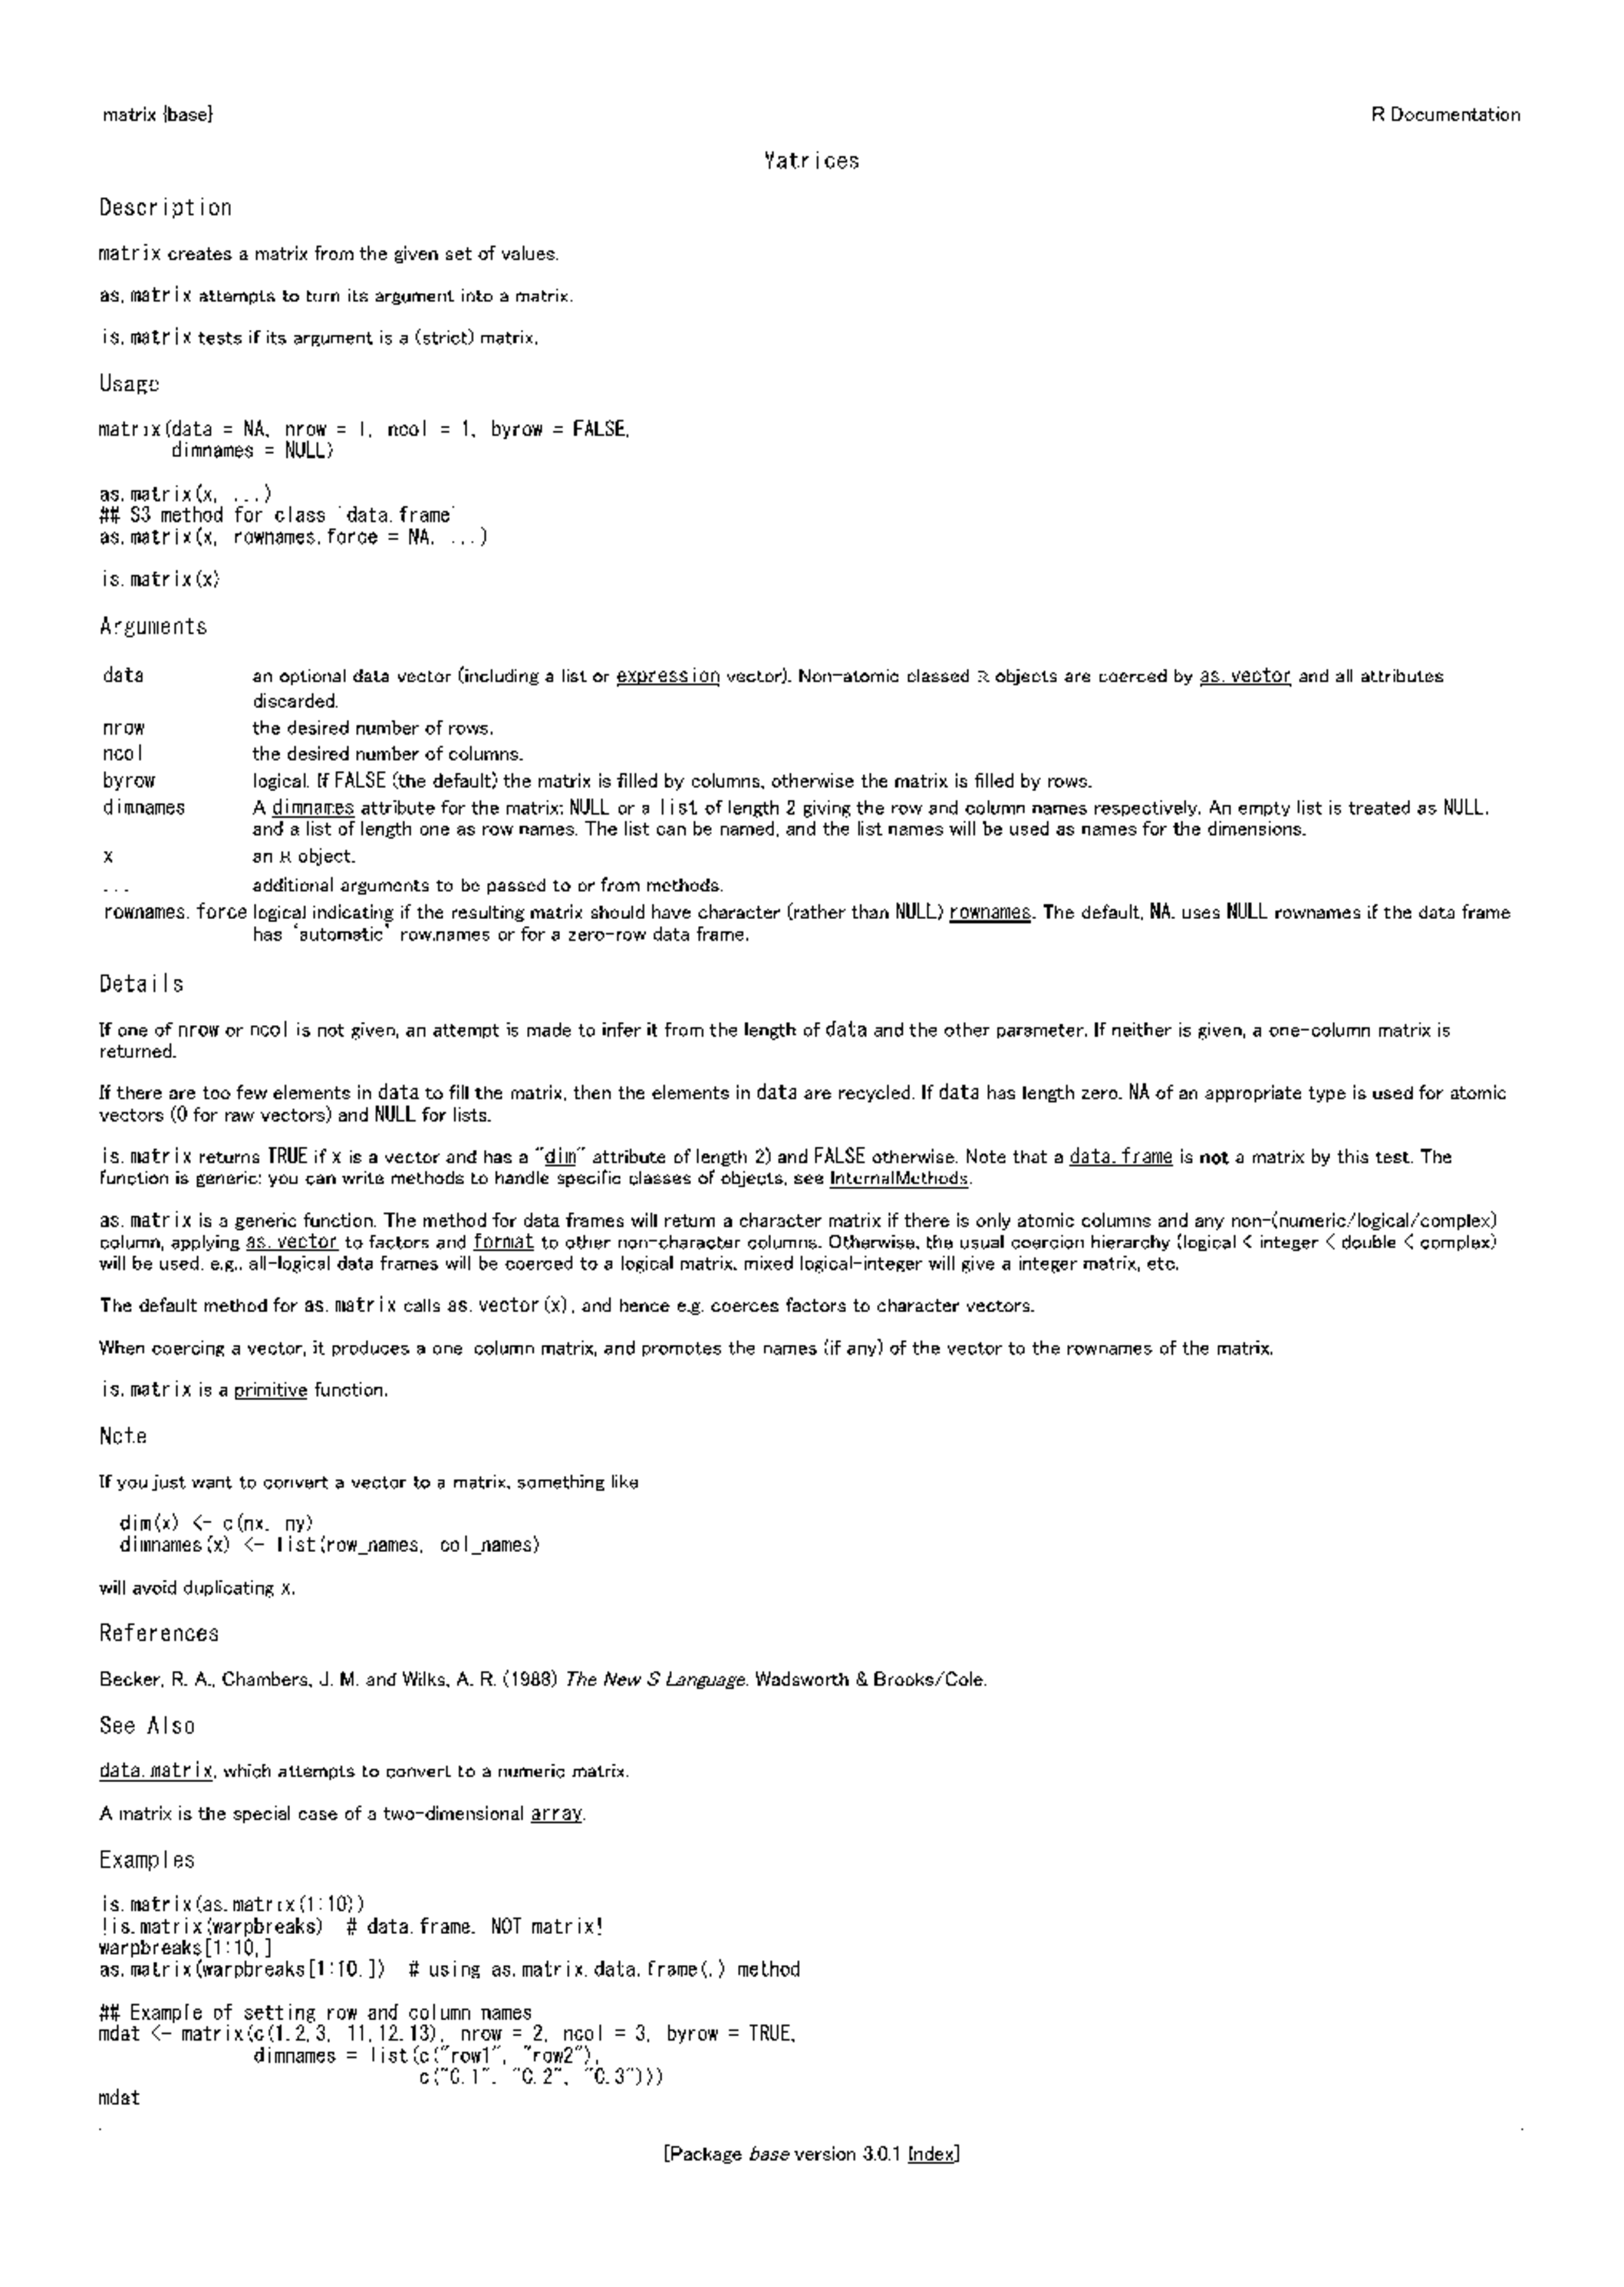
\includegraphics[height=15cm]{img/matrices.eps}
\end{center}

\subsection{便利に使う}
Rではコンソール画面の他にエディタ画面も用意されている.Macの場合は画面上部のアイコンをクリックして画面を表示する.\\
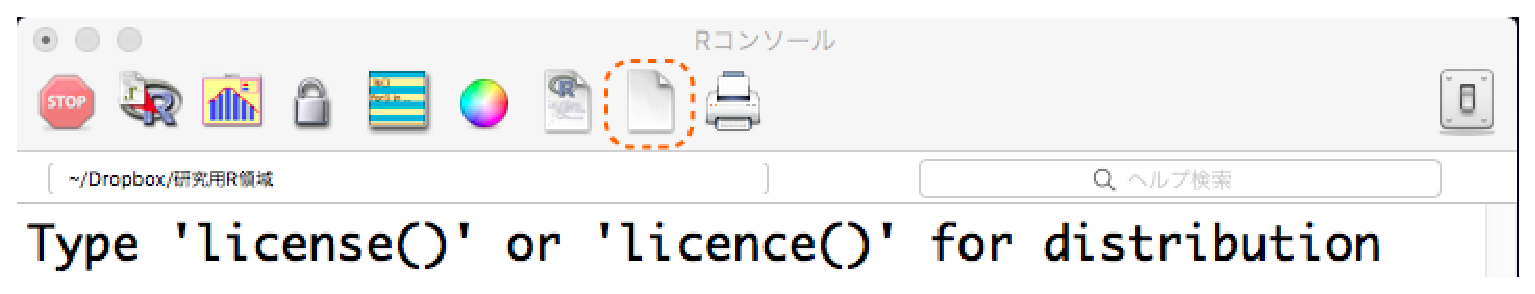
\includegraphics[width=10cm]{img/maceditor.eps}\\
Windowsの場合は上部メニューのファイル>新しいスクリプトをクリックする.\\
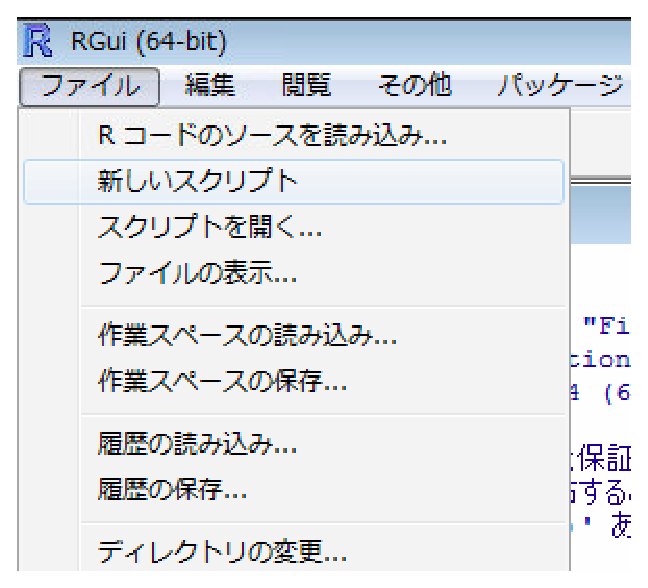
\includegraphics[width=7cm]{img/wineditor.eps}

エディタ画面では,編集した内容を \kbd{Ctrl} + \kbd{R} や \kbd{
\includegraphics[height=0.9em]{img/commandKey.eps} Command} + \kbd{Enter} で選択した部分はキャレット(カーソル)がある行を実行することができる.

また,コンソール画面では関数名・オブジェクト名を打っている途中でTABキーを押すと候補が表示される.
\subsection{オブジェクトの管理と設定}
\subsubsection{オブジェクトの型を変換する}
オブジェクトには様々な型やデータ構造がある.確認するには\verb+class(オブジェクト名)+や\verb+str(オブジェクト名)+などの関数での確認が必要な場合がある.
\begin{breakbox}
\begin{verbatim}
> class(iris)
[1] "data.frame"
> str(iris)
'data.frame':   150 obs. of  5 variables:
 $ Sepal.Length: num  5.1 4.9 4.7 4.6 5 5.4 4.6 5 4.4 4.9 ...
 $ Sepal.Width : num  3.5 3 3.2 3.1 3.6 3.9 3.4 3.4 2.9 3.1 ...
 $ Petal.Length: num  1.4 1.4 1.3 1.5 1.4 1.7 1.4 1.5 1.4 1.5 ...
 $ Petal.Width : num  0.2 0.2 0.2 0.2 0.2 0.4 0.3 0.2 0.2 0.1 ...
 $ Species     : Factor w/ 3 levels "setosa","versicolor",..: 1 1 1 1 1 1 1 1 1 1 ...
> iris$Petal.Length=as.factor(iris$Petal.Length)
> str(iris)
'data.frame':   150 obs. of  5 variables:
 $ Sepal.Length: num  5.1 4.9 4.7 4.6 5 5.4 4.6 5 4.4 4.9 ...
 $ Sepal.Width : num  3.5 3 3.2 3.1 3.6 3.9 3.4 3.4 2.9 3.1 ...
 $ Petal.Length: Factor w/ 43 levels "1","1.1","1.2",..: 5 5 4 6 5 8 5 6 5 6 ...
 $ Petal.Width : num  0.2 0.2 0.2 0.2 0.2 0.4 0.3 0.2 0.2 0.1 ...
 $ Species     : Factor w/ 3 levels "setosa","versicolor",..: 1 1 1 1 1 1 1 1 1 1 ...
\end{verbatim}
\end{breakbox}
このように型を変更することができる.
\begin{description}
\item[型の確認や変更の関数]\mbox{}
\begin{table}[H]
\begin{center}
% \caption{表}
\vspace{1zw}
\label{03AB-A2}
\begin{tabular}{c|l|l}
\noalign{\hrule height 1pt}
&\multicolumn{1}{c|}{型の確認}&\multicolumn{1}{c}{変換}\\ \hline
実数&\verb+is.numeric()+&\verb+as.numeric()+\\
整数&\verb+is.integer()+&\verb+as.integer()+\\
複素数&\verb+is.complex()+&\verb+as.complex()+\\
文字列&\verb+is.character()+&\verb+as.character()+\\
論理値&\verb+is.logical()+&\verb+as.logical()+\\
\noalign{\hrule height 1pt}
\end{tabular}
\end{center}
\end{table}
\item[データ構造の確認や変更の関数]\mbox{}
\begin{table}[H]
\begin{center}
% \caption{表}
\vspace{1zw}
\label{03AB-A2}
\begin{tabular}{c|l|l}
\noalign{\hrule height 1pt}
&\multicolumn{1}{c|}{構造の確認}&\multicolumn{1}{c}{変換}\\ \hline
ベクトル&\verb+is.vector()+&\verb+as.vector()+\\
行列&\verb+is.matrix()+&\verb+as.matrix()+\\
配列&\verb+is.array()+&\verb+as.array()+\\
リスト&\verb+is.list()+&\verb+as.list()+\\
データフレーム&\verb+is.data.frame()+&\verb+as.data.frame()+\\
順序なし因子&\verb+is.factor()+&\verb+as.factor()+\\
順序つき因子&\verb+is.ordered()+&\verb+as.ordered()+\\
\noalign{\hrule height 1pt}
\end{tabular}
\end{center}
\end{table}
\end{description}

これらの{\tt is}で始まる関数は,{\tt TRUE や FALSE}を返す.また,データの内容を確認したい場合は{\tt head}関数や{\tt tail}関数を使用する.この関数はデータの上から,もしくは下から6つ分のデータを表示する関数である.
\begin{breakbox}
\begin{verbatim}
> head(iris)
  Sepal.Length Sepal.Width Petal.Length Petal.Width Species
1          5.1         3.5          1.4         0.2  setosa
2          4.9         3.0          1.4         0.2  setosa
3          4.7         3.2          1.3         0.2  setosa
4          4.6         3.1          1.5         0.2  setosa
5          5.0         3.6          1.4         0.2  setosa
6          5.4         3.9          1.7         0.4  setosa
> tail(iris)
    Sepal.Length Sepal.Width Petal.Length Petal.Width   Species
145          6.7         3.3          5.7         2.5 virginica
146          6.7         3.0          5.2         2.3 virginica
147          6.3         2.5          5.0         1.9 virginica
148          6.5         3.0          5.2         2.0 virginica
149          6.2         3.4          5.4         2.3 virginica
150          5.9         3.0          5.1         1.8 virginica
\end{verbatim}
\end{breakbox}
\subsubsection{データの中の変数を呼び出す}
前述のとおりデータの中の変数を使う場合には\verb+data$var+というような使い方を書いたが,実際には指定することが面倒になる場合がある.その場合,{\tt attach}関数を用いてそのまま変数を使用することができる.
\begin{breakbox}
\begin{verbatim}
> head(Sepal.Length)
 以下にエラー head(Sepal.Length) :  オブジェクト 'Sepal.Length' がありません 
> attach(iris)
> head(Sepal.Length)
[1] 5.1 4.9 4.7 4.6 5.0 5.4
\end{verbatim}
\end{breakbox}
使い終わったら,{\tt detach}関数で解除することをお奨めする.
\begin{breakbox}
\begin{verbatim}
> detach(iris)
> head(Sepal.Length)
 以下にエラー head(Sepal.Length) :  オブジェクト 'Sepal.Length' がありません 
\end{verbatim}
\end{breakbox}
\subsubsection{作成したオブジェクトの削除}
続けて使用しているとオブジェクトが不必要になることがある.その場合,オブジェクトを消去すればよい.
\begin{breakbox}
\begin{verbatim}
> ls()
[1] "chuo"   "debian" "ubuntu"
> objects()
[1] "chuo"   "debian" "ubuntu"
> rm(debian)
> ls()
[1] "chuo"   "ubuntu"
> rm(list = ls(all = TRUE))
> ls()
character(0)
\end{verbatim}
\end{breakbox}
{\tt ls}関数や{\tt objects}関数でオブジェクトを確認できる.{\tt rm}関数で個別に消去もでき,全消去することもできる.また,メニューより全消去することも可能だ.

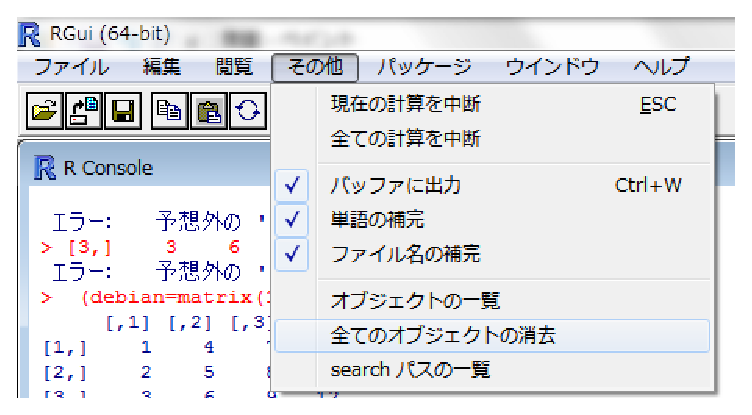
\includegraphics[height=4cm]{img/windows/rmall.eps}\hspace{0.8em} 
\includegraphics[height=4cm]{img/windows/honki.eps}
\subsection{基本的な関数}
ここでは,主に使用する関数を一部抜粋して記す.
\begin{table}[H]
\begin{center}
% \caption{表}
\vspace{1zw}
\begin{tabular}{l|l}
\noalign{\hrule height 1pt}
\multicolumn{1}{c|}{関 数}&\multicolumn{1}{c}{種 類}\\ \hline
\verb+c(x1,x2,...)+ &配列(ベクトルの作成)\\
\rowcolor{bl} \verb+rep(x,times)+ &{\tt x}を{\tt times}回繰り返す\\
\verb+seq(初項, 末項, 公差)+ &等差数列の作成\\
\rowcolor{bl} \verb+matrix(c(x1, x2, ...),行数, 列数, byrow = FALSE)+ &行列の作成 ({\tt byrow}は配列を列方向に代入する引数)\\
\verb+abs(x)+ &絶対値\\
\rowcolor{bl} \verb+mean(x)+ &平均\\
\verb+var(x)+ &分散\\
\rowcolor{bl} \verb+median(x)+ &中央値\\
\verb+max(x)+ &最大値\\
\rowcolor{bl} \verb+min(x)+ &最小値\\
\verb+cor(x,y)+ &相関係数\\
\rowcolor{bl} \verb+t()+&行列の転置\\
\verb+solve(x)+&逆行列の生成\\
\rowcolor{bl} \verb+eigen(x)+ &固有値と固有ベクトル\\
\verb+sqrt(x)+ &平方根\\
\rowcolor{bl} \verb+exp(x)+ &指数関数\\
\verb+log(x, base = exp(1))+ &{\tt base}を底とした対数\\
\rowcolor{bl} \verb+sum(x)+ &総和\\
\verb+cumsum(x)+ &累積和\\
\rowcolor{bl} \verb+prod(x)+ &総乗\\
\verb+cumprod(x)+ &累積積\\
\rowcolor{bl} \verb+sin(x)+ &正弦関数\\
\verb+floor(x)+ &切り捨て\\
\rowcolor{bl} \verb+ceiling(x)+ &切り上げ\\
\verb+round(x, digits = 0)+ &整数に丸める\\
\rowcolor{bl} \verb+length(x)+ &ベクトルの長さを調べる\\
\verb+dim(x)+ &行列やデータフレームの行数と列数を調べる\\
\noalign{\hrule height 1pt}
\end{tabular}
\end{center}
\end{table}
引数に数値やベクトル,行列を入れることによって計算結果を得ることができる.1つの数値を入力する関数にベクトルや行列を代入すると,Rでは要素ごとに計算を行う.
\subsubsection{確率分布}
Rでは乱数発生アルゴリズムが存在する.併せて確率密度関数や累積分布関数の計算もできるので覚えておくとよい.
\begin{table}[H]
\begin{center}
% \caption{表}
\vspace{1zw}
\begin{tabular}{l|l}
\noalign{\hrule height 1pt}
\multicolumn{1}{c|}{種類}&\multicolumn{1}{c}{関数}\\ \hline
確率密度関数&{\tt d*(確率点)}\\
累積分布関数&{\tt p*(確率点)}\\
確率点(累積分布関数の逆関数)&{\tt q*(確率)}\\
乱数発生&{\tt r*(個数)}\\
\noalign{\hrule height 1pt}
\end{tabular}
\end{center}
\end{table}

以下では主な確率分布を取り上げる.引数に初期値が設定されているものもある.
\begin{table}[H]
\begin{center}
% \caption{表}
\vspace{1zw}
\begin{tabular}{l||l|l}
\noalign{\hrule height 1pt}
\multicolumn{1}{c||}{確率分布}&\multicolumn{1}{c|}{関数}&\multicolumn{1}{c}{引数}\\ \hline
一様分布&{\tt unif}&{\tt min = 0, max = 1}\\
二項分布&{\tt binom}&{\tt size, prob}\\
正規分布&{\tt norm}&{\tt mean = 0, sd = 1}\\
ポアソン分布&{\tt pois}&{\tt lambda}\\
指数分布&{\tt exp}&{\tt rate = 1}\\
$\chi^2$分布&{\tt chisq}&{\tt df, ncp = 0}\\
\noalign{\hrule height 1pt}
\end{tabular}
\end{center}
\end{table}

つまり,一様分布$U(0,1)$において,$P(X=0.5)$の確率を求めたい場合は\verb+dunif(0.5)+,$P(X < 0.5)$を求めたい場合は\verb+punif(0.5)+,$P(X < y)=0.5$となる$y$を求める場合は\verb+qunif(0.5)+,この一様分布に従う乱数を10個生成したい場合は\verb+runif(10)+となる.
\subsection{作図}
ここでは,{\tt plot}関数を用いて作図を行う.\\
基本形は{\tt plot(x, y)}もしくは{\tt plot(y \verb+~+ x)}である.変数が一つでもよい.オプション引数を特に指定しない場合は,自動で適当な作図してくれる.
\begin{screen}
\verb+plot(x, y, type = "", xlab = "", ylab = "", main = "", sub = "", xlim = c(, ), ylim = c(, ), axes = TRUE, pch = "", col = "", lty = "", lwd = "", ...)+ 
\end{screen}
引数を指定しない場合は自動で初期値となる.
\subsubsection{軸}
\begin{description}
\item[軸の表示] \mbox{}\\
{\tt axes = FALSE}とした場合,図の枠や軸は表示されない.\\
その場合,あとから{\tt box()}関数で枠を書くことができる.
\begin{screen}
{\tt box()}
\end{screen}
後から軸を書く場合は,{\tt axis()}関数を使用する.
\begin{screen}
\begin{verbatim}
axis(1) # 下の軸を表示する 2:左,3:上,4:右
axis(1, at = c(0.4, 0.6, 0.9)) # 引数 at を用いて軸の任意の箇所に数字を表示することも可能だ.
\end{verbatim}
\end{screen}
\item[表題] \mbox{}\\
表題は{\tt main},サブタイトルは{\tt sub}で指定する.文字列は\verb+""+で指定すること.作図後に表題を追加する場合は{\tt title()}関数を使用する.
\begin{screen}
\begin{verbatim}
title(main = "表題", sub = "サブタイトル")
\end{verbatim}
\end{screen}
\item[X軸,Y軸の名前] \mbox{}\\
{\tt xlab}と{\tt ylab}で指定する.同様に,後から追加する場合は{\tt title}関数を使用する.
\begin{screen}
\begin{verbatim}
title(xlab = "X軸の名前", ylab = "Y軸の名前")
\end{verbatim}
\end{screen}
\item[X軸,Y軸の上限と下限] \mbox{}\\
{\tt xlim = c(上限, 下限)},{\tt ylim = c(上限, 下限)}で指定する.
\end{description}
\subsubsection{種類}
{\tt type}で指定する.以下はRの標準で用意されているグラフの一覧である.
\begin{table}[H]
\begin{center}
% \caption{表}
\vspace{1zw}
\label{03AB-A2}
\begin{tabular}{c|l}
\noalign{\hrule height 1pt}
指定&\multicolumn{1}{c}{種類}\\ \hline
\verb+type = "p"+ &点プロット(2変数でのデフォルト)\\
\verb+type = "l"+ &線プロット(折れ線グラフ・1変数でのデフォルト)\\
\verb+type = "b"+ &点と線のプロット\\
\verb+type = "c"+ &\verb+"b"+ において点を描かないプロット\\
\verb+type = "o"+ &点プロットと線プロットの重ね書き\\
\verb+type = "h"+ &各点からx 軸までの垂線プロット\\
\verb+type = "s"+ &左側の値にもとづいて階段状に結ぶ\\
\verb+type = "S"+ &右側の値にもとづいて階段状に結ぶ\\
\verb+type = "n"+ &軸だけ描いてプロットしない(続けて低水準関数でプロットする場合)\\
\noalign{\hrule height 1pt}
\end{tabular}
\end{center}
\end{table}

また,点をプロットする場合プロット記号を指定することができる.\verb+pch+で指定する.
\begin{center}
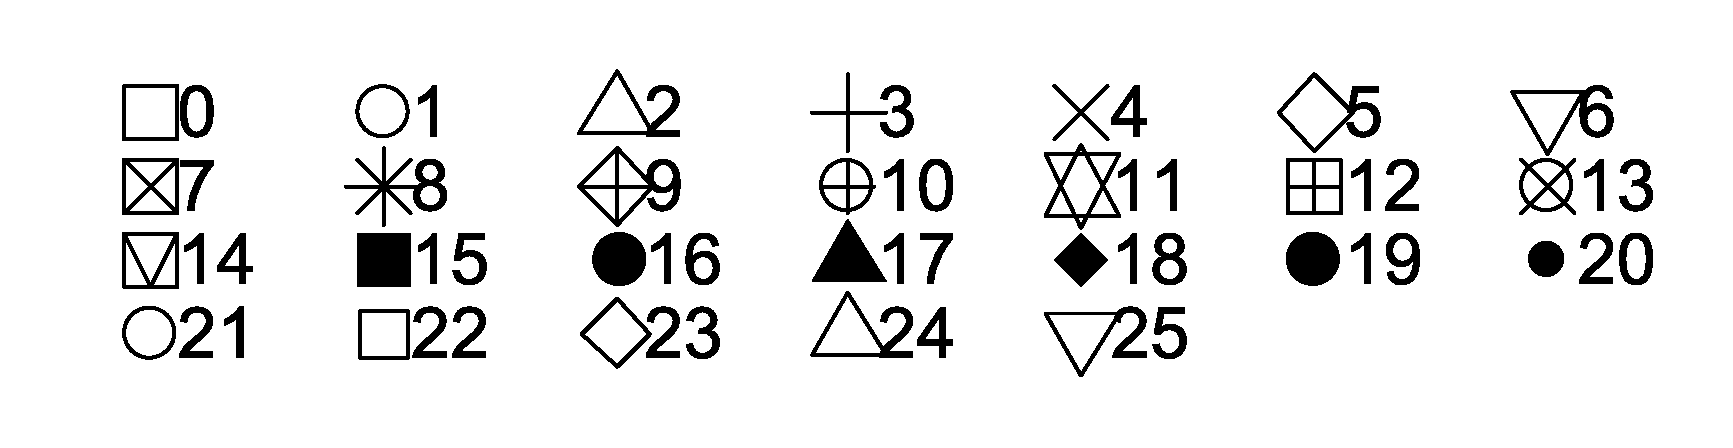
\includegraphics[height=2cm]{img/pch.eps}
\end{center}

なお,プロット記号の大きさは,\verb+cex+で指定する.線をプロットする場合,線の種類({\tt lty})や線の幅({\tt lwd})を指定することができる.
\begin{figure}[H]
  \begin{center}
    \begin{tabular}{c}
      % 1
      \begin{minipage}{0.3\hsize}
        \begin{center}
          \verb+lty+で線の種類の指定\\
          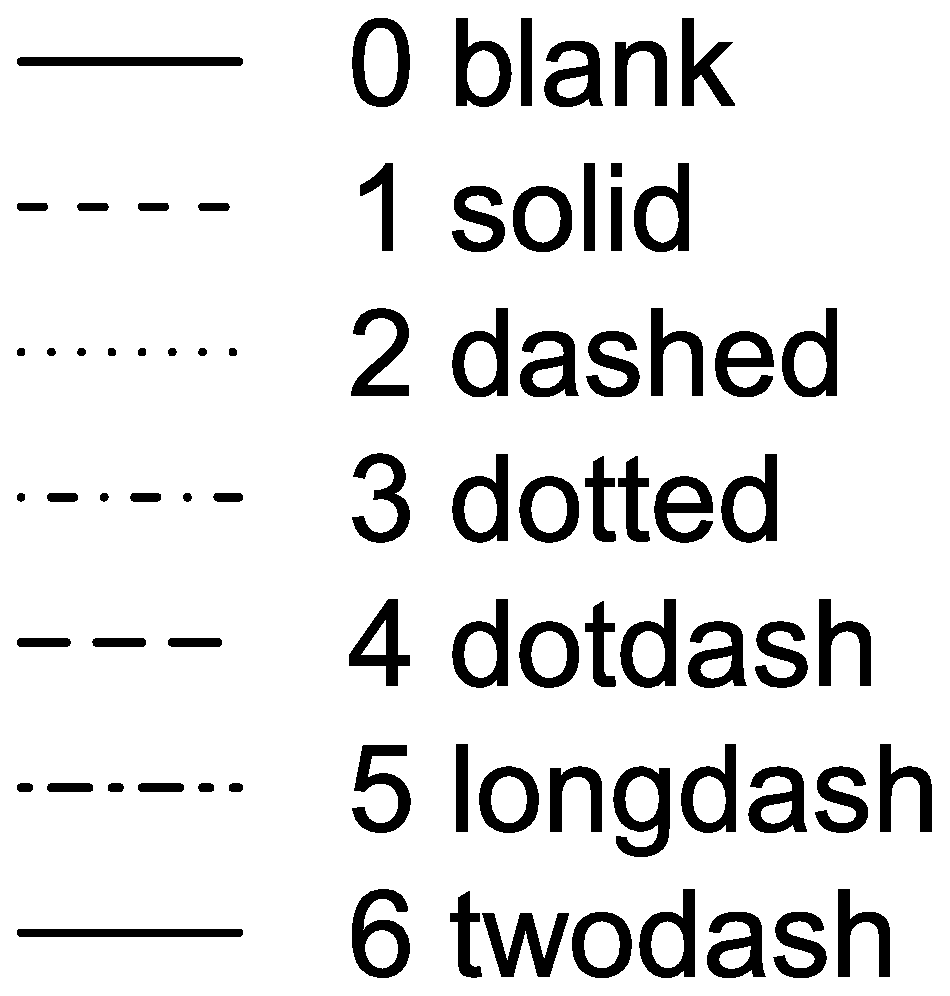
\includegraphics[height=2.5cm]{img/lty.eps}
        \end{center}
      \end{minipage}
      % 2
      \begin{minipage}{0.3\hsize}
        \begin{center}
          \verb+lwd+で線の太さの指定\\
          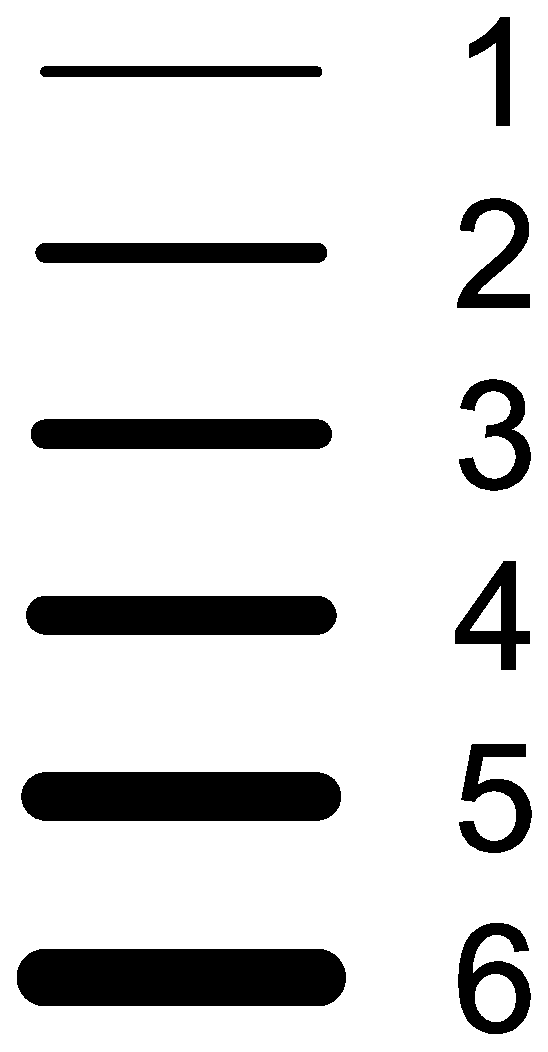
\includegraphics[height=2.5cm]{img/lwd.eps}
        \end{center}
      \end{minipage}
    \end{tabular}
  \end{center}
\end{figure}

他にも,色を変えることもできる.
\begin{table}[H]
\begin{center}
% \caption{表}
\vspace{1zw}
\label{03AB-A2}
\begin{tabular}{c||c|l}
\noalign{\hrule height 1pt}
色&番号&\multicolumn{1}{c}{名前}\\ \hline
■&\tt 1&\tt black\\
\textcolor{myred}{■}&\tt 2&\tt red\\
\textcolor{mygreen}{■}&\tt 3&\tt green\\
\textcolor{myblue}{■}&\tt 4&\tt blue\\
\textcolor{mycyan}{■}&\tt 5&\tt cyan\\
\textcolor{mymagenta}{■}&\tt 6&\tt magenta\\
\textcolor{myyellow}{■}&\tt 7&\tt yellow\\
\textcolor{bl}{■}&\tt 8&\tt gray\\
\noalign{\hrule height 1pt}
\end{tabular}
\end{center}
\end{table}

16進数でRGBを指定することや,\verb+colors()+関数を使用して,Rに定義されている657色を選択することも可能である.
\begin{breakbox}
\begin{verbatim}
> head(colors())
[1] "white"         "aliceblue"     "antiquewhite"  "antiquewhite1"
[5] "antiquewhite2" "antiquewhite3"
> plot(lynx, col = colors()[25])
> plot(lynx, col = "#8080FF")
\end{verbatim}
\end{breakbox}
{\tt pch}や{\tt col}に\verb+c(1, 1, 2, 1, 1)+と指定すれば,任意の箇所だけを色を変えたり,記号を変えることもできる.\\
また,{\tt lines()}や{\tt points()},{\tt abline()}関数を使用して,先ほどのプロットに点や線を重ねて書くこともできる.
\begin{screen}
\begin{verbatim}
abline(v = 15) # x=15 に縦の直線を引く
abline(h = 20, col = 2) # y = 20に横の直線を引く
\end{verbatim}
\end{screen}

Windows では表示されたグラフを右クリックすることで保存することや Microsoft Office Word に貼り付けることができる.




\noindent
{\bf \large{Macでの作図}}

Macで作図をする場合,文字が□に化けてしまう.(この□はネット上では豆腐と呼ばれる)そのため作図前に{\tt par}関数を用いて設定を変更するか,
\begin{screen}
\begin{verbatim}
par(family="HiraKakuProN-W3").
\end{verbatim}
\end{screen}
\verb+~/.Rprofile+を作成する必要がある.
\begin{screen}
\begin{verbatim}
setHook(packageEvent("grDevices", "onLoad"),
	function(...){
        if(.Platform$OS.type == "windows")
            grDevices::windowsFonts(sans ="MS Gothic",
                                    serif="MS Mincho",
                                    mono ="FixedFont")
        if(capabilities("aqua"))
            grDevices::quartzFonts(
              sans =grDevices::quartzFont(
                c("Hiragino Kaku Gothic Pro W3",
                  "Hiragino Kaku Gothic Pro W6",
                  "Hiragino Kaku Gothic Pro W3",
                  "Hiragino Kaku Gothic Pro W6")),
              serif=grDevices::quartzFont(
                c("Hiragino Mincho Pro W3",
                  "Hiragino Mincho Pro W6",
                  "Hiragino Mincho Pro W3",
                  "Hiragino Mincho Pro W6")))
        if(capabilities("X11"))
            grDevices::X11.options(
                fonts=c("-kochi-gothic-%s-%s-*-*-%d-*-*-*-*-*-*-*",
                        "-adobe-symbol-medium-r-*-*-%d-*-*-*-*-*-*-*"))
        grDevices::pdf.options(family="Japan1GothicBBB")
        grDevices::ps.options(family="Japan1GothicBBB")
        }
)

attach(NULL, name = "JapanEnv")
assign("familyset_hook",
       function() {
            winfontdevs=c("windows","win.metafile",
                          "png","bmp","jpeg","tiff")
            macfontdevs=c("quartz","quartz_off_screen")
            devname=strsplit(names(dev.cur()),":")[[1L]][1]
            if ((.Platform$OS.type == "windows") &&
                (devname %in% winfontdevs))
                    par(family = "sans")
            if (capabilities("aqua") &&
                devname %in% macfontdevs)
                    par(family = "sans")
       },
       pos="JapanEnv")
setHook("plot.new", get("familyset_hook", pos = "JapanEnv"))
setHook("persp", get("familyset_hook", pos = "JapanEnv"))
\end{verbatim}
\end{screen}
面倒だし,やり忘れた人は\verb+plot+時に\verb+family = "Osaka"+ としておけばとりあえず表示には困らない.

\subsection{関数の定義}
基本的な形式はこの形である.(入力した引数を)演算子し,{\tt return()}で返す.
\begin{screen}
\begin{verbatim}
myfunc <- function(x){
  a = x%%2
  return(a)
}
\end{verbatim}
\end{screen}
\subsubsection{条件分岐(if文)}
\begin{screen}
\begin{verbatim}
myfunc <- function(x){
  a = x%%2
  if(a == 0){
    return(TRUE) # a == 0 が真の場合の処理
  }else if(a == 1){
    return(FALSE) # a == 0 が偽の場合で a == 1 が真の場合の処理
  }else{
    return("Not Integer") # a == 0 が偽の場合で a == 1 が偽の場合の処理
  }
}
\end{verbatim}
\end{screen}
この定義した関数で計算した結果が以下である.
\begin{breakbox}
\begin{verbatim}
> myfunc(1)
[1] FALSE
> myfunc(2)
[1] TRUE
> myfunc(2.1)
[1] "Not Integer"
\end{verbatim}
\end{breakbox}

なお,比較演算子や論理演算子は以下である.
\begin{description}
\item[比較演算子]\mbox{}
\begin{center}
\begin{tabular}{c|c}
\noalign{\hrule height 1pt}
演算子&\multicolumn{1}{c}{意味}\\ \hline
\verb+==+&$=$\\
\verb+!=+&$\ne$\\
\verb+>+&$>$\\
\verb+<+&$<$\\
\verb+>=+&$\geq$\\
\verb+<=+&$\leq$\\
\noalign{\hrule height 1pt}
\end{tabular}
\end{center}
\item[論理演算子]\mbox{}
\begin{center}
\begin{tabular}{c|lc}
\noalign{\hrule height 1pt}
演算子&\multicolumn{2}{c}{意味}\\ \hline
\verb+!+&否定&$\lnot$\\
\verb+&&+&論理積(かつ) &$ \land $ \\
\verb+||+&論理和(または) &$ \lor $ \\
\verb+xor()+&排他的論理和 &$\oplus$ \\
\noalign{\hrule height 1pt}
\end{tabular}
\end{center}
\end{description}

以下のように,比較演算だけを行うこともできる.また,ベクトルで演算を行えばベクトルの要素ごとの演算結果を返してくれる.
\begin{breakbox}
\begin{verbatim}
> 2==3
[1] FALSE
> 2 == 3 || 5 == 5
[1] TRUE
> c(1, 2, 3) != c(3, 2, 1)
[1]  TRUE FALSE  TRUE
\end{verbatim}
\end{breakbox}

また,オブジェクトから条件に合うものだけを抽出したり,条件に合うオブジェクト内の要素の番号を得ることもできる.
\begin{breakbox}
\begin{verbatim}
> b = 11:30
> b[b %% 2 == 0] # bを2で割った余りが0の要素を表示
 [1] 12 14 16 18 20 22 24 26 28 30
> which(b %% 2 == 0) # bを2で割った余りが0の要素の番号を表示
 [1]  2  4  6  8 10 12 14 16 18 20
\end{verbatim}
\end{breakbox}
\subsubsection{繰り返し(for分とwhile文)}
\begin{screen}
\begin{verbatim}
for(i in 1:10){
  #関数
  print(i)
 }
# 1:10ではなく任意のベクトルにしてもよい.
# この場合 i を変数として使える.

while (x <= 5) { # while ( 条件式 )
  x <- x + 1
  # 条件式が TRUE である限り式が繰り返される
} 

\end{verbatim}
\end{screen}
\subsection{パッケージの利用}
前述のとおり,Rには多くのパッケージが存在している.パッケージを使用することで,解析手法や関数を導入することができる.
\begin{breakbox}
\begin{verbatim}
> install.packages("ismev") # ライブラリのインストール
 パッケージを 'C:/Users/User/Documents/R/win-library/2.15' 中にインストールします 
 ('lib' が指定されていないので) 
 --- このセッションで使うために,CRANのミラーサイトを選んでください --- 
 URL 'http://cran.rstudio.com/bin/windows/contrib/2.15/ismev_1.39.zip' を試しています 
Content type 'application/zip' length 192211 bytes (187 Kb)
 開かれた URL 
downloaded 187 Kb

 パッケージ 'ismev' は無事に展開され,MD5 サムもチェックされました 

 ダウンロードされたパッケージは,以下にあります 
        C:\Users\User\AppData\Local\Temp\Rtmp2BJBEa\downloaded_packages 
\end{verbatim}
\end{breakbox}
これで,パッケージのインストールは完了した.メニューより選択してインストールすることも可能だ.

インストールしたパッケージを呼び出すには,\verb+library+関数を使用する.
\begin{breakbox}
\begin{verbatim}
> library(ismev) # ライブラリの呼び出し
 要求されたパッケージ mgcv をロード中です 
This is mgcv 1.7-18. For overview type 'help("mgcv-package")'.
 警告メッセージ: 
 パッケージ ''ismev'' はバージョン 2.15.3 の R の下で造られました 
\end{verbatim}
\end{breakbox}
またコマンドではなくメニューからパッケージをインストールする方法もある.
\begin{figure}[H]
  \begin{center}
    \begin{tabular}{c}
      % 1
      \begin{minipage}{0.4\hsize}
        %\begin{center}
          メニューの``パッケージ"から\\``パッケージのインストール"を選択し,\\
          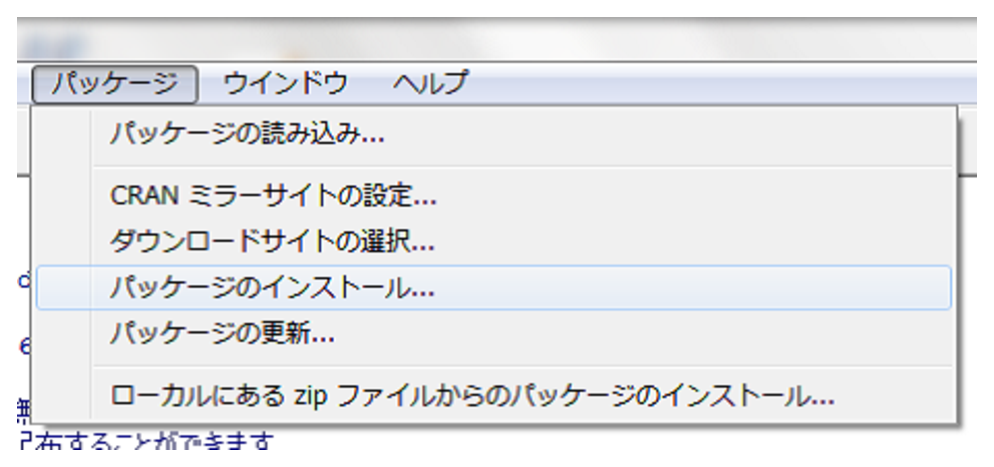
\includegraphics[height=2.5cm]{img/pkg1.eps}\\ \\ \\ \\ \\ \\ \\ \\ \\ \\ \\ \\ \\ \\
        %\end{center}
      \end{minipage}
      % 2
      \begin{minipage}{0.3\hsize}
        %\begin{center}
          CRANのミラーサーバを選択し,\\
          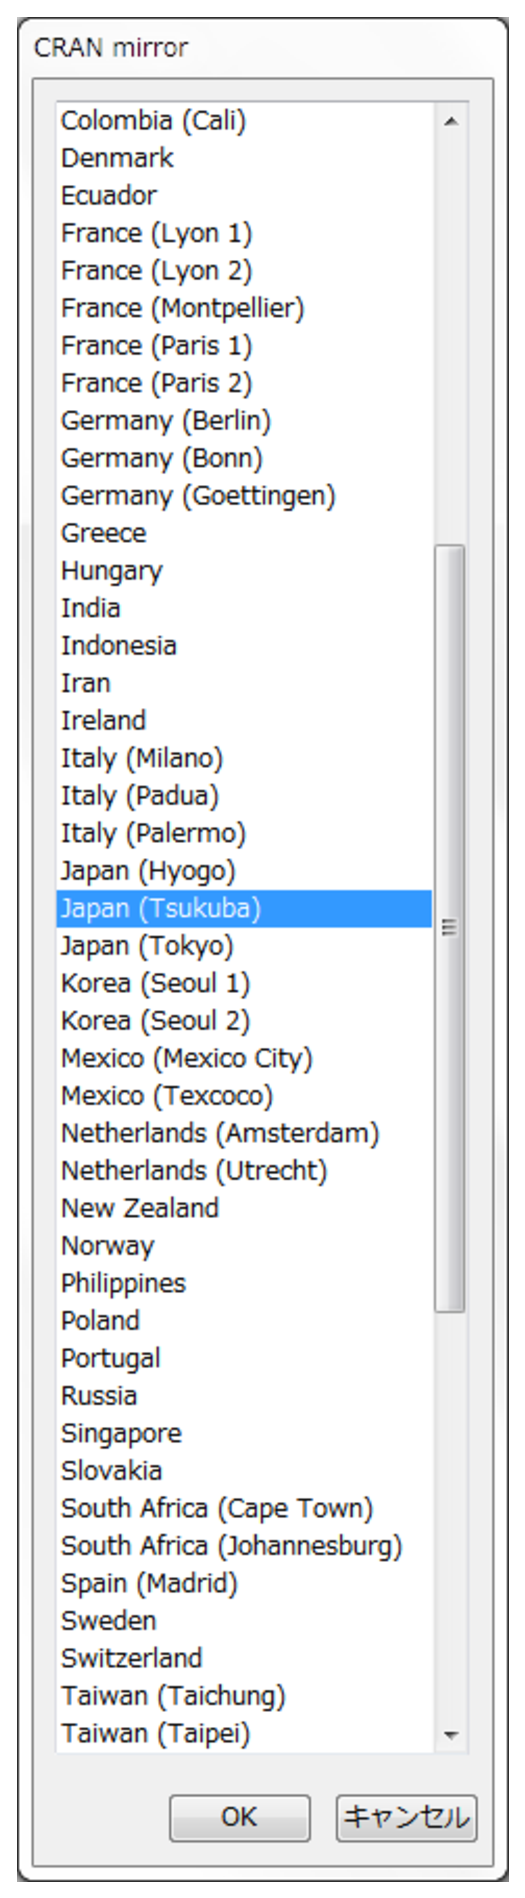
\includegraphics[height=10cm]{img/pkg2.eps}\\

        %\end{center}
      \end{minipage}
      % 3
      \begin{minipage}{0.3\hsize}
        %\begin{center}
          パッケージ一覧から選択するとインストールされる.\\
          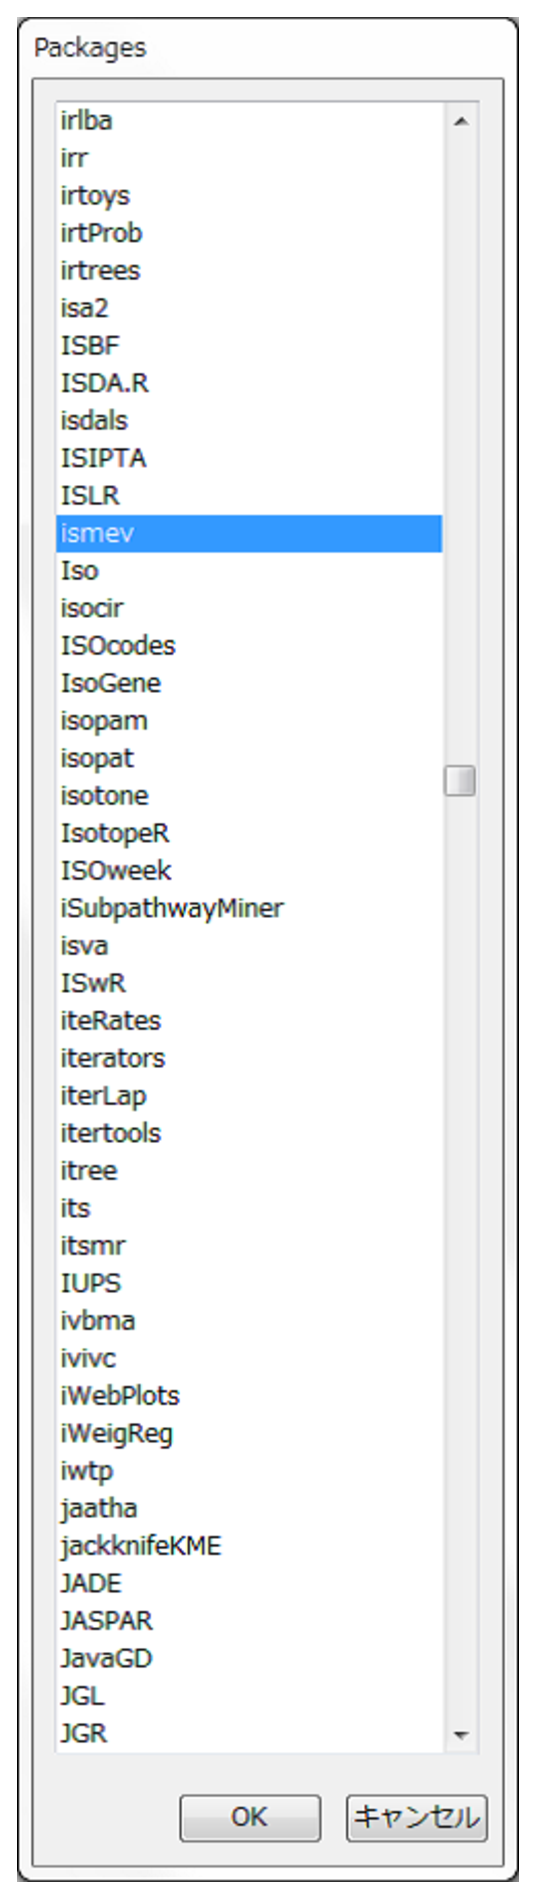
\includegraphics[height=10cm]{img/pkg3.eps}
        %\end{center}
      \end{minipage}
    \end{tabular}
  \end{center}
\end{figure}
\subsection{よくある失敗と対処法}
\subsubsection{プロキシ設定}
研究室のLAN回線ではプロキシサーバーを経由した環境である場合が多い.その場合,Rのパッケージをダウンロードできないため,設定が必要である.
\begin{description}
\item [(Windowsのみ)ショートカットからプロキシの設定の場合]\mbox{}\\
\begin{figure}[H]
  \begin{center}
    \begin{tabular}{c}
      % 1
      \begin{minipage}{0.35\hsize}
        %\begin{center}
          ショートカットを右クリックし,\\プロパティ(R)を開く.\\
          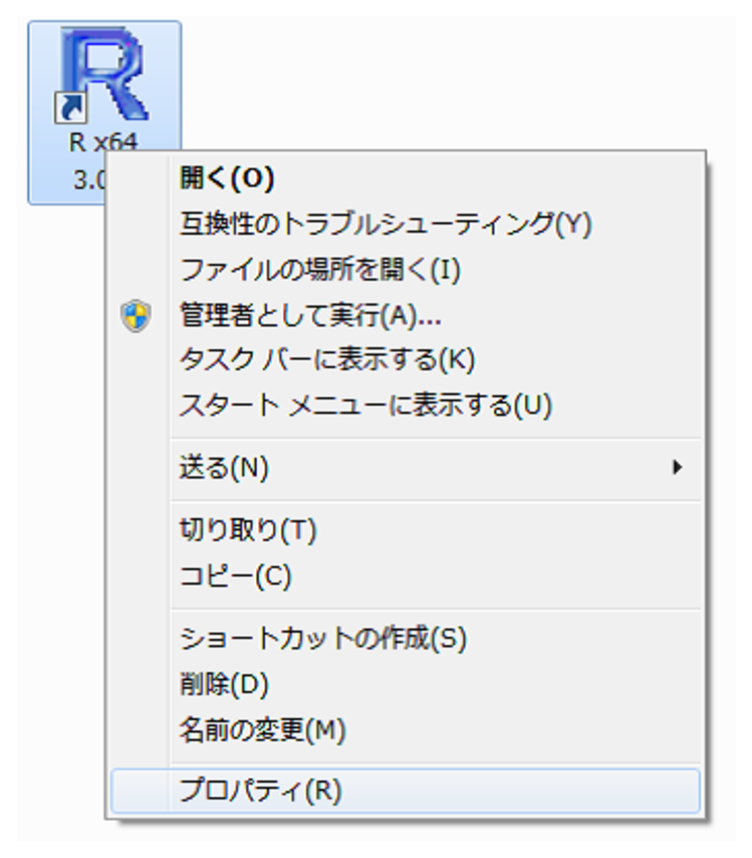
\includegraphics[width=6cm]{img/migi.eps}\\ \\ \\ \\ \\
        %\end{center}
      \end{minipage}
      % 2
      \begin{minipage}{0.65\hsize}
        %\begin{center}
          リンク先(T)のパスの後ろに,\verb+ [スペース]--internet2+を追加し,\\
          \verb+"C:\Program Files\R\R-3.0.1\bin\x64\Rgui.exe --internet2"+\\
          にする.\\
          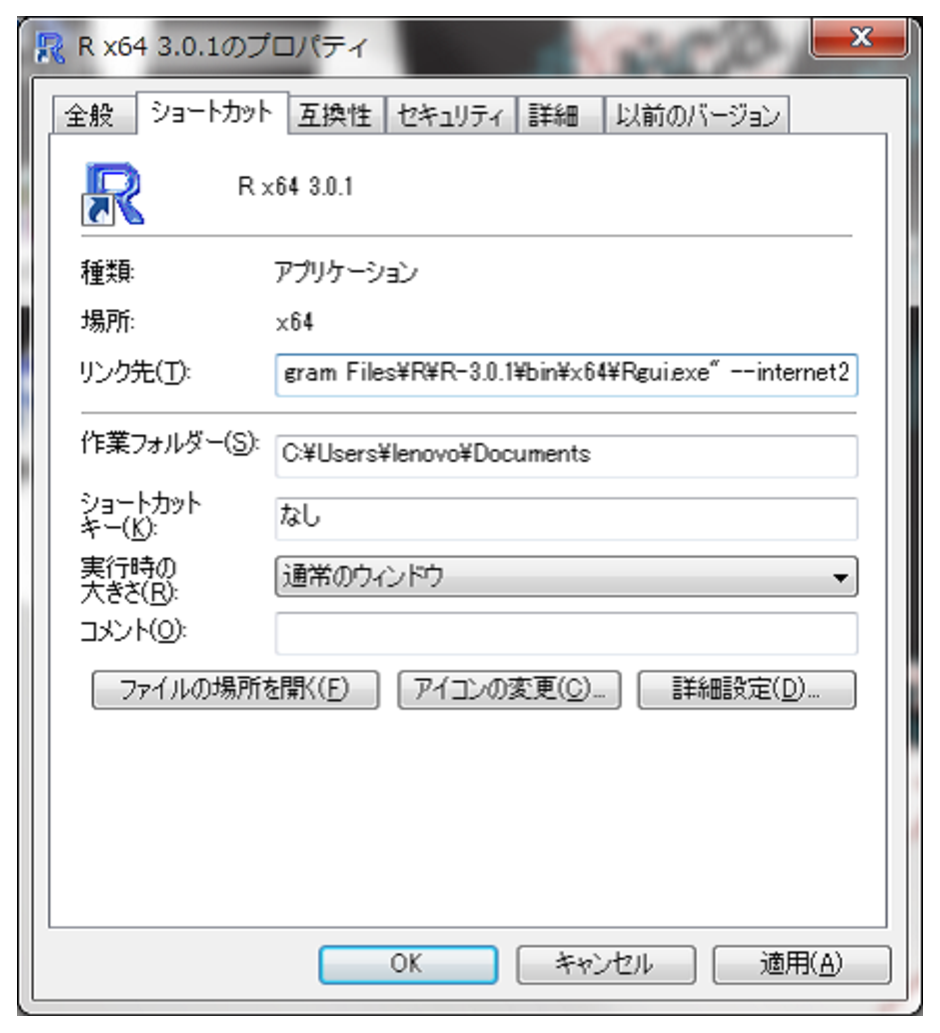
\includegraphics[width=8.2cm]{img/property.eps}
        %\end{center}
      \end{minipage}
    \end{tabular}
  \end{center}
\end{figure}
\item[(すべてのOS)コマンドで設定の場合]\mbox{}\\
最近では暗号化されたセキュアなサーバも増えてきているので1行目だけでなく2行目の\verb+https_proxy+も忘れないようにしたい.
\begin{screen}
\begin{verbatim}
Sys.setenv("http_proxy" = "http://サーバーアドレス:ポート番号")
Sys.setenv("https_proxy" = "http://サーバーアドレス:ポート番号")
\end{verbatim}
\end{screen}
\end{description}
\subsubsection{入力エラー}
また,下の例ように閉じの\verb+"+や\verb+)+を入力せずにEnterを押すと,次の閉じの記号まで,入力待ちになってしまう.この場合,閉じの記号を入力してEnterを押すか,Escを押して先ほどの入力をキャンセルすることができる.
\begin{breakbox}
\begin{verbatim}
> tmp = "university
+ 
\end{verbatim}
\end{breakbox}